\chapter{Hypernymy Detection and Asym}\label{ch:lexmem}

This chapter introduces the Asym model and related material. The work
in this chapter has been published in \newcite{roller:2014:coling}.

\section{Chapter Overview}

Automatically identifying lexical relationships is a long standing task
in NLP \cite{hearst:1992:coling,snow:2004:nips,girju:2006:cl}, which has
implications for textual entailment, question answering, information
retrieval, and more. Hypernymy, or an is-a relationship like \lit{cat} is an
animal, is of particular interest for many applications. Most approaches tend
to focus on identifying specific lexico-syntactic patterns which are indicative
of particular relations, but require that direct observation of words in
those patterns. The use of distributional vectors holds promise of increasing
recall over lexico-syntactic patterns, but the literature has focused mostly
on unsupervised measures with limited success.

We propose Asym, a novel {\em supervised} model for automatically identifying
hypernymy using distributional vectors. Our measure draws inspiration from
the Distributional Inclusion Hypothesis \cite{zhitomirskygeffet:2005:acl},
which states that the contexts in which \lit{animal} may appear should be a
superset of the contexts in which \lit{cat} may appear. We propose a novel
experimental setup to measure how well models generalize to unseen lexical
items, and show that our model performs well in these adversarial experimental
conditions.

\section{Prior Work}

There is a large body of work on automatically extracting word relationships
from unannotated corpora, and thus it is nearly impossible to cover all work
exhaustively. Nonetheless, we here try to sketch out some of the main branches
of research which have led to our own work.

One of the seminal works in automatic hypernymy discovery was that of Hearst
patterns \cite{hearst:1992:coling}. Hearst showed that certain lexico-syntactic
idioms were very clear indicators of hypernymy relationships. Some example
Hearst patterns are \lit{animals such as cats}; \lit{animals for example cats};
and \lit{animals including cats}. Each of these provides evidence that \lit{animal} is a
hypernym of \lit{cat}, especially when the pattern is repeated several times across a
large corpus \cite{hearst:1992:coling}. With a strong set of patterns, and a
large enough corpus, many hypernymy relationships may easily be captured.

Unfortunately, such patterns can be brittle and sensitive to minor inflections
or variations.  These patterns above would fail to also capture the
relationship between \lit{animals} and \lit{dogs} if provided \lit{animals, such as cats and dogs}. Some work
has sought to address these issues by expanding the lists of Hearst
patterns and increasing coverage by using
rough frequency estimates from web search engines (e.g. Google, Bing) rather
than explicit counts \cite{seitner:2016:lrec}. Others generalize known patterns
over Part-of-Speech tags \cite{sang:2007:acl} or language models
\cite{ritter:2009:aaai}. These efforts can greatly improve on the low recall
of Hearst patterns with relatively small sacrifices in precision.

\begin{figure}
\centering
\begin{dependency}[edge vertical padding=0.5ex, edge style={black},
                  label style={fill=black,text=white,font=\ttfamily}]
  \begin{deptext}[column sep=0.7cm,nodes={font=\large}]
    animals, \& such \& as \& cats \& and \& dogs\\
  \end{deptext}
  \depedge{1}{3}{prep}
  \depedge{3}{2}{mwe}
  \depedge{3}{4}{pobj}
  \depedge{4}{5}{cc}
  \depedge{5}{6}{conj}
\end{dependency}\\
{\small (a) vanilla dependency parse}\\~\\
\begin{dependency}[edge vertical padding=0.5ex, edge style={black},
                  label style={fill=black,text=white,font=\ttfamily}]
  \begin{deptext}[column sep=0.7cm,nodes={font=\large}]
    animals, \& such as \& cats \& dogs \\
  \end{deptext}
  \depedge{1}{2}{prep}
  \depedge{2}{3}{pobj}
  \depedge{2}{4}{pobj}
\end{dependency}\\
{\small (b) collapsed dependency parse}\\
\caption{(a) Dependency parse for ``Animals, such
  as cats and dogs,'' and (b) The collapsed dependency parse of the same
\cite{marneffe:2008:techreport}.}
\label{fig:collapseddep}
\end{figure}

Another line of work seeks to generalize Hearst patterns from word patterns
to syntactic patterns. \newcite{snow:2004:nips}, in particular, showed that
using patterns over syntactic parses can greatly improve the representational power,
and significantly improve both precision and recall. For example,
Figure~\ref{fig:collapseddep} shows how a dependency parse can be lightly
processed so that the conjunction \lit{and} no longer stands between
\lit{animals} and \lit{dog}, and the multiword expression (MWE) \lit{such as}
is collapsed to a single node. Later work by \newcite{snow:2006:acl} shows
this can be improved further by jointly identifying many relations in a
taxonomy at a single time. However, even with improvements through joint
relationship identification and more patterns, one limitation of Hearst
patterns is that words {\em must} co-occur together explicitly using one of
the patterns. This limitation, combined with the success of distributional
vector space models, has led to the question: can distributional methods be
used for identifying lexical relationships? And if so, what can their
success teach us about distributional methods?

\subsection{Distributional Approaches}
\label{sec:dih}

Much of the earlier work in applying distributional approaches to lexical
entailment detection focused primarily on {\em unsupervised} methods, positing
that relationships should be apparent through regular behavior across the
dimensions of a sparse vector space. The reasoning went that with the
right entailment similarity measure, one could measure the
entailment-similarity between any two words and estimate the degree to which
one word entailed another. This would occur in the same way that cosine
similarity can tell you the degree to which two words are related. Crucially,
the hypothetical {\em entails} measure {\em must} in general be asymmetric,
\begin{equation*}
  \mbox{entails}(\vu, \vv) \neq \mbox{entails}(\vv, \vu),
\end{equation*}
or any two entailing terms (e.g. \lit{cat} $\rightarrow$ \lit{animal}) will
also entail the converse \mbox{(\lit{animal} $\rightarrow$ \lit{cat})}.

One of the first approaches was that of \newcite{weeds:2004:coling}, who
introduced the notion of \emph{distributional generality}, where $v$ is
distributionally more general than $u$ if the $u$ appears in a subset of the
contexts in which $v$ is found, as illustrated in Figure~\ref{fig:dih}.  They
speculate that hypernyms should be more distributionally general than hyponym,
and measure distributional generality using a variation of
precision~\cite{weeds:2003:emnlp,weeds:2004:coling}:
\begin{align}
  1(x) & = \begin{cases}1 & \mbox{if } x > 0\\
    0 & \mbox{otherwise}
  \end{cases}\\
  \mbox{WeedsPrec}(\vu, \vv) & = \frac{\sum_{i=1}^n u_i * 1(v_i)}{\sum_{i=1}^n u_i}
  \label{eq:weeds}
\end{align}
Intuitively, {\WeedsPrec} computes the number of contexts of $u$ which are also
a part of $v$, and weights each context by its importance to $u$. Note that
the weights of contexts in $v$ are {\em not} considered, only their absence
or presence.

\newcite{geffet:2004:coling,zhitomirskygeffet:2005:acl} point out that generic
distributional similarity is too loose for precision-demanding applications
like Question Answering or Textual Entailment, and that the definition should
be changed slightly. They propose the {\em Distributional Inclusion Hypothesis}
(DIH), which states that a {\em lexical entailment} relation holds between two
words when ``one of the words can be substituted by the other
[word], such that the meaning of the original word can be inferred from the new
one'' \cite{zhitomirskygeffet:2005:acl}. The DIH generalizes the view of
distributional generality beyond hypernymy and provides a more rigorous
definition.  Figure~\ref{fig:dih} illustrates the DIH, emphasizing that the
contexts in which \lit{cat} appears should be a subset of the contexts in which
\lit{animal} appears. Meanwhile, under this interpretation, co-hyponyms should
have a high degree of overlapping contexts.

\begin{figure}
\centering
\begin{tikzpicture}[scale=0.75\textwidth/12.0cm]
    \coordinate (cat) at (-1.0,0);
    \coordinate (dog) at ( 1.0,0);
    \coordinate (animal) at (0,0);
    \def \catcircle{(cat) circle (2.5)}
    \def \dogcircle{(dog) circle (2.5)}

    \draw [fill=Gray, fill opacity=0.3] (0,0.5) circle (4.0);
    \draw [fill=Cerulean] \dogcircle;
    \draw [fill=Goldenrod] \catcircle;
    \begin{scope}
      \clip \catcircle;
      \draw [fill=Cerulean, fill opacity=0.5] \dogcircle;
    \end{scope}
    % full universe box
    \draw [ultra thick] (-6,-4) rectangle (6,6);

    % labels
    \draw (-2.5,0) node[align=center] {\word{cat}\\contexts};
    \draw ( 2.5,0) node[align=center] {\word{dog}\\ contexts};
    \draw (origin) node[align=center] {\word{cat} \& \word{dog}\\ contexts};
    \draw (0,3.25) node[align=center] {\word{animal} contexts};
    \draw (0,5.25) node[align=center] {all contexts};
\end{tikzpicture}
\caption{Illustration of the Distributional Inclusion Hypothesis (DIH)
  \cite{zhitomirskygeffet:2005:acl}, which hypothesizes that the contexts in
  which \lit{cat} appears should be a subset of the contexts in which
  \lit{animal} appears. Co-hyponyms are hypothesized to have overlapping, but
  distinct contexts.}
\label{fig:dih}
\end{figure}

To this end, \newcite{kotlerman:2010:nle} introduces a dataset for lexical
entailment and propose the distributional similarity measure {\balAPinc}
predicting lexical entailment.  The {\balAPinc} measure is a modification of
the Average Precision (AP) measure from Information Retrieval. The general
notion is that scores should increase both with the number of included
features, and give more weight to the highly ranked features of the narrower
term $u$. This is captured by computing the number of included features at
every rank $P(r), r\in\{1,\ldots,|W|\}$, and weighting by the corresponding
rank in the broader term, $rel'(f_r)$. The final measure, {\balAPinc} smooths
using the well known {\em LIN} similarity measure \cite{lin:1998:icml}:
\begin{align}
  \mbox{APinc}(\vu, \vv) & = \frac{\sum_{r=1}^{|1(\vu)|}P(r)\cdot rel'(f_r))}{|1(\vu)|}\\
  \mbox{balAPinc}(\vu, \vv)  & = \sqrt{\mbox{APinc}(\vu, \vv)\cdot \mbox{LIN}(\vu, \vv)}
\end{align}

Another measure proposed in the same vein is {\Clarke} \cite{clarke:2009:gems},
which takes inspiration from \newcite{weeds:2004:coling}, but also considers
the {\em degree} to which a term $v$ is contained within $u$ by evaluating
over a component-wise minimum. Intuitively, this allows us to measure
distributional inclusion beyond mere presence or absence (as in \WeedsPrec),
and consider the degree to which {\em important} contexts are included.
\begin{equation}
  \mbox{CL}(\vu, \vv) = \frac{\sum_{i=1}^n \mbox{min}(u_i, v_i)}{\sum_{i=1}^n u_i}
\end{equation}

\newcite{lenci:2012:starsem} introduce the \mbox{\invCL} measure which uses
{\Clarke} to measure both distributional inclusion of $u$ in $v$ and
distributional non-inclusion of $v$ in $u$. While all other measures interpret
the Distributional Inclusion Hypothesis as the degree to which a $\subseteq$
relation holds, \newcite{lenci:2012:starsem} test the degree to which proper
inclusion $\subsetneq$ holds. They consider not only the degree to which the
contexts of the narrower terms are included in the contexts of the wider term,
but also determine the degree to which the wider term has contexts that the
narrower term does not have, and balance the two terms using a geometric mean:
\begin{equation}
    \mbox{invCL}(\vu, \vv) = \sqrt{\mbox{CL}(\vu, \vv) * (1 - \mbox{CL}(\vv, \vu))}
  \label{eq:invcl}
\end{equation}

A few other unsupervised approaches, not based on the DIH, have also been
proposed. In particular, \newcite{santus:2014:eacl} introduce the SLQS measure,
which computes a transformed distributional space by weighting contexts via
their overall entropy \cite{shannon:1948:bell}. For any given two terms
$u$ and $v$, the final measure depends on distribution of their top-$k$ entropy
values, reasoning that the narrower term should have less entropy in its
contexts.  Follow up studies found the SLQS measure is sensitive to
hyperparameter tuning (namely, selection of $k$, the number of contexts to
consider), but outperforms other measures with careful tuning
\cite{shwartz:2017:eacl}.

\paragraph{Evaluating Unsupervised Measures}

We motivate our work with an original comparison of the available measures
based on the DIH (Equations~\ref{eq:weeds}--\ref{eq:invcl}) on their ability to
separate hypernymy from three other relations: co-hyponymy, meronymy, and
random. We also include cosine similarity as a scientific control.
We evaluate using the BLESS dataset \cite{baroni:2011:gems},
which contains annotations of word relations for 200 mostly unambiguous, concrete
nouns like \lit{van}, \lit{horse}, and \lit{chair}. These concepts are divided
into 17 general Categories, like \lit{vehicle}, \lit{ground mammal} and
\lit{furniture}. Each noun is annotated with its co-hyponyms, meronyms,
hypernyms and some random pairs. The original dataset additionally contains
some additional verb relations, but we use only the noun-noun relationships,
totally about 14k data points.

We compute the similarity between the LHS and RHS for each pair in BLESS using
each of the measures.  We then compute the Average Precision for each concept
and relation types, and reported the Mean Average Precision (MAP) across all
200 concepts.  Table~\ref{tab:mapscores1} shows these MAP scores for the
different relations and measures. An ideal {\em entails} measure would have a
MAP of $1.0$ in the Hyper column, and $0.0$ in other columns.

\begin{table}
  \centering
  \begin{small}
  \begin{tabular}{|l|cccc|}
    \hline
    Measure        & Co-hyp  & Hyper  & Mero  & Random  \\
    \hline
    cosine         &   .68   &   .20  &  .27  &    .27  \\
    balAPinc       &   .56   &   .23  &  .31  &    .28  \\
    WeedsPrec      &   .52   &   .22  &  .33  &    .28  \\
    Clarke         &   .66   &   .19  &  .28  &    .28  \\
    invCL          &   .60   &   .18  &  .31  &    .28  \\
    \hline
  \end{tabular}
  \end{small}
  \caption{Mean Average Precision (MAP)  for the unsupervised entailment
    measures on the BLESS dataset. An ideal measure has a MAP of $1.0$ in the
    Hyper column and $0.0$ in the other columns. All measures fail to select
    hypernymy with greater precision than co-hyponymy.}
  \label{tab:mapscores1}
\end{table}

Overall, we find none of the measures give an actively higher score for the
hypernymy relation than the other three relations, indicating a dramatic
failure of all the chosen measures. Indeed, two of the measures even (slightly)
underperform cosine similarity. This raises the question: are the measures
just overly sensitive to noise in distributional vectors, or is the
Distributional Inclusion Hypothesis fundamentally flawed? If the unsupervised
are measures are simply too sensitive to noise, perhaps using supervised
techniques can improve performance. To this end, we shift our attention to
{\em supervised} methods, hypothesizing that they will be more robust to
the noise of distributional vectors.

\section{Importance of Experimental Conditions}

As we turn our attention to supervised methods , we first consider how
experimental setup can significantly impact performance and yield misleading
results.

As with all supervised machine learning methods, it is important to create
distinct {\em training} and {\em testing} splits of the data. The training
split is used to learn any model parameters, while the testing split is used to
evaluate a model's generalization by checking that the model is able to make
predictions on {\em unseen} data. Traditional methods for creating train/test
splits of data are simple randomization (80\% for train, 20\% for test,
stochastically assigning each data item to one or the other). When a particular
dataset is somewhat small, it is often common to evaluate using
cross-validation (CV), where the data is split into $k$ equal sized {\em folds}
and then each fold is used as the test set in $k$ separate evaluations.
Typically the performance metric (like accuracy) is averaged across all $k$
folds.  When the $k$ in cross-validation is taken to be the full dataset size,
then we arrive at a Leave-one-out cross-validation (LOOCV) experimental setup.

As with other datasets, we can evaluate our hypernymy datasets using any of
these setups. For example, we could randomly assign 80\% of the word pairs in
our dataset as training, and utilize the remaining 20\% as testing. However, due the
construction of the different datasets, many words appear multiple times in the
dataset: sometimes they appear on the LHS, sometimes on the RHS, and always
annotated with several example relationships. This means if we
separate our training and testing data using standard random splits, then
sometimes particular words will appear both in training and in test splits, and
we may have issue generalizing to new pairs containing unseen words.
Table~\ref{tab:splits}a demonstrates this issue in an example, toy dataset.
Crucially, we see that in this toy example, three words appear in both the
training and testing sets.

To remedy this, we propose a variation of LOOCV where an individual {\em
concept} is withheld as a particular test set, and the training set consists of
all the remaining pairs which do not contain any lexical overlap. For example,
if \mbox{(cat,~animal)} appears in our test set, then the test set will consist
of all \mbox{(cat,~*)} pairs, and all \mbox{(*,~animal)} pairs will be
discarded from the training set. This adversarial experimental setup ensures
that we can truly ensure our model is able to identify the lexical relationship
of novel pairs, and not simply memorizing certain words.
Table~\ref{tab:splits}b demonstrates our setup.

\begin{table}
  \hfill
  \begin{minipage}[b]{0.49\textwidth}
  \centering
  \begin{maybesmall}
  \begin{tabular}{|llll|}
    \hline
    {\bf LHS} & {\bf RHS} & {\bf Category} & {\bf Label} \\
    \hline
    \hline
    \multicolumn{4}{|c|}{Test set}\\
    \hline
    cat       &  animal   &  mammal        & hyper       \\
    sofa      &  tooth    &  furniture     & rand        \\
    \hline
    \hline
    \multicolumn{4}{|c|}{Training set}\\
    \hline
    dog       &  animal   &  mammal        & hyper       \\
    dog       &  cat      &  mammal        & co-hyp      \\
    dog       &  book     &  mammal        & rand        \\
    cat       &  desk     &  mammal        & rand        \\
    sofa      &  chair    &  furniture     & hyper       \\
    \hline
  \end{tabular}\\~\\{(a) random split}
  \end{maybesmall}
  \end{minipage}
  \hfill
  \begin{minipage}[b]{0.49\textwidth}
    \centering
  \begin{maybesmall}
  \begin{tabular}{|llll|}
    \hline
    {\bf LHS} & {\bf RHS} & {\bf Category} & {\bf Label} \\
    \hline
    \hline
    \multicolumn{4}{|c|}{Test set}\\
    \hline
    cat       &  animal   &  mammal        & hyper       \\
    cat       &  desk     &  mammal        & rand        \\
    \hline
    \hline
    \multicolumn{4}{|c|}{Training set}\\
    \hline
    dog       &  book     &  mammal        & rand        \\
    sofa      &  chair    &  furniture     & hyper       \\
    sofa      &  tooth    &  furniture     & rand        \\
    \hline
    \hline
    \multicolumn{4}{|c|}{Discarded}\\
    \hline
    dog       &  animal   &  mammal        & hyper       \\
    dog       &  cat      &  mammal        & co-hyp      \\
    \hline
  \end{tabular}\\~\\{(b) our split}
  \end{maybesmall}
  \end{minipage}
  \hfill
  \caption{(a) An example randomized train/test set split for a toy dataset.
  Note how the words \lit{cat}, \lit{animal}, and \lit{sofa} appear in both
  training and testing sets. (b) Our chosen splitting of the same data. Notice
  no words appear in both training and in test, but some pairs will necessarily
  be discarded.}
\label{tab:splits}
\end{table}

Unfortunately, one downside of this setup is that some pairs must be discarded
in each particular train/test setup, as shown in the Dropped section of
Table~\ref{tab:splits}b. This will occur in any dataset where a particular word
occurs in more than one example pair.  This can be mitigated by keeping the
size of each test set to its smallest reasonable value to minimize the
possibility of overlap with other pairs. Figure~\ref{fig:dataloss} shows the
percentage of training data that must be discarded on two different datasets.
A traditional machine learning setup, where no pairs are discarded because
overlap is disregarded, would lie at the $y = 0.0$ line. We see that the
amount of data that must be discarded rapidly increases with the size of
the test set due to the increased vocabulary coverage; indeed, in a basic
ten-fold CV setting, we need to discard 83\% of the BLESS training data, and
in three-fold CV we must discard 99\%. We conclude that using many small
folds is better for data efficiency, though this also comes at a computational
cost, since we must run our classifiers for many more trials.

\begin{figure}
  \centering
  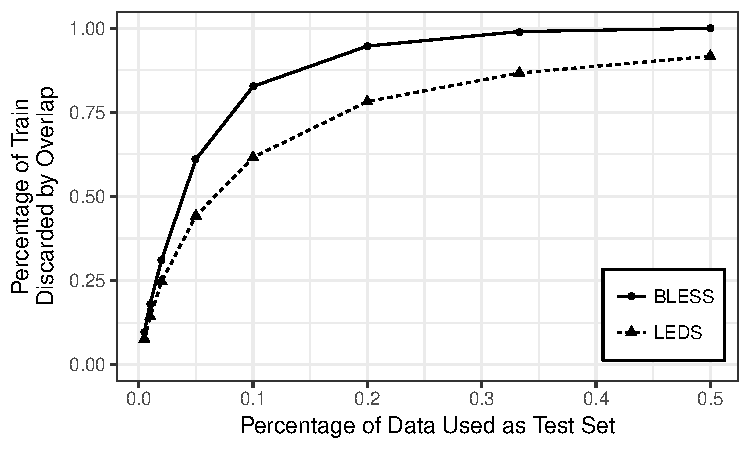
\includegraphics[width=0.75\textwidth]{plots/foldloss}
  \caption{The amount of training data that must be eliminated by removing pairs
    sharing words in common between training and test, as a function of test
    set size. As the test set size increased, the number of overlapping pairs
    increases rapidly.}
  \label{fig:dataloss}
\end{figure}

A third evaluation setting can also exist for the BLESS dataset, which contains
additional annotations of {\em Category} along with each concept. These
17 high-level categories include \lit{ground mammal}, \lit{fruit},
\lit{amphibian/reptile}, \lit{furniture} and \lit{musical instrument}. Thus,
we may also consider leave-out-one-{\em Category} CV.

We compare these three evaluation settings (traditional, LOO Concept, and LOO
Category) by training and evaluating a fixed, existing supervised model.
Namely, we use the model of \newcite{baroni:2012:eacl}, who use an
off-the-shelf SVM with a polynomial kernel, reasoning that a polynomial SVM is
able to capture the importance of features and their interactions
\cite{cortes:1995:ml}. Following their work, we use the concatenation of the
raw vectors of a dimensionality-reduced, small-window, bag-of-words
distributional space for input features. That is, for our running
example, we use the features,
\begin{equation*}
  \mbox{features}(\vv, \vu) = [\litvec{cat}; \litvec{animal}].
\end{equation*}
Table~\ref{tab:overlapresults} shows the accuracy of this
classifier with these features on the four-way classification task
of BLESS, both with lexical overlap and without lexical overlap. We did not
evaluate a random split setting without lexical overlap.

\begin{table}
  \centering
  \begin{tabular}{|l|c|c|}
      \hline
      {\bf Stratification} & {\bf W/ overlap} & {\bf W/o overlap} \\
      \hline
      \hline
      Random               &   .976           &     -             \\
      Concept (LHS)        &   .971           &   .765            \\
      Category             &   .710           &   .652            \\
      \hline
  \end{tabular}
  \caption{Comparing experimental conditions with and without lexical overlap
    on the classifier proposed by \newcite{baroni:2012:eacl}.}
  \label{tab:overlapresults}
\end{table}

One clear pattern from these results is a substantial
decrease in performance when switching from allowing lexical overlap to
removing lexical overlap: the concept-level stratification performance drops
by over 20 points, and the category stratification drops by nearly 6 points.
This substantial decrease shows one of our major observations: that some
classifiers may be prone to a special form of overfitting, where random pairs
like (\lit{cactus},~\lit{animal}) are classified as hypernymy, because the
model simply {\em memorizes} that \lit{animal} is always a hypernym when it
appears on the RHS, or that \lit{cactus} is always a hyponym when it appears
on the LHS.

This discovery of memorization was simultaneously published by both
\newcite{roller:2014:coling} and \newcite{weeds:2014:coling}, but each chose to
deal with the issue in separate ways. The former controlled for memorization
using the concept-level stratification we describe above, while the latter
controlled for by comparing models with a randomized control variant, which
used {\em random} vectors to represent each word. Models which had little
difference between their real and randomized results were assumed to be
memorizing the data, while models which improved over random vectors were
considered strong. This is a very different approach to controlling for
lexical memorization. We consider this setup to be inadequate, since
randomized vectors are unable to exploit the distributional hypothesis, and
therefore systematically underestimate the robustness of some models.

Our second observation is that stratification by category is substantially
more difficult than stratification by concept, regardless of whether or
not lexical overlap is allowed. The reason for this is threefold:
(1) Stratification by category already accounts for a large percentage over
lexical overlap, as many of the overlapping pairs are drawn from the same
high-level categories. (2) Since there are only 17 categories, but 200 concepts,
this moves us from 200-fold CV to 17-fold CV, causing our training set sizes
to be significantly smaller (\texttildelow99\% vs \texttildelow88\% of the full
data). This is exacerbated when disallowing lexical overlap, as it moves us
significantly further along the curve shown in Figure~\ref{fig:dataloss}.
(3) Category-level stratification changes the problem into a sort of
domain-transfer setting, where we must learn about lexical relationships in
the domain of mammals and then generalize to relationships about
furniture, thus making the task markedly harder, as one must consider
that the co-occurrences of \lit{cat} and \lit{stool} will likely overlap
very little.

Clearly, the choice of experimental setup yields vastly different pictures of
how well a model generalizes to new data. Evaluating with zero lexical overlap
is important if we wish to distinguish between a model which truly generalizes
to novel words and one which simply memorizes the data. Category stratification
is important when we are interested in generalizing models to new domains;
unfortunately, category information is only available in one dataset, making
it difficult to test robustness of models across multiple datasets.

On the other hand, \newcite{shwartz:2016:acl} argue that allowing lexical
overlap is possibly more realistic, since lexicographers are more likely to
want to insert words into an existing and incomplete ontology, rather than
induce entirely new ontologies from scratch. In our own work, we hope to learn
about what kinds of entailment signals are available in distributional
vectors, and what these signals tell us about lexical relationships, rather
than absolute performance on ontology completion. Therefore, we consider
concept-level stratification with zero lexical overlap to be most appropriate
for our own research. Since the models we consider in this chapter are
computationally inexpensive, we employ a Leave-out-one-Concept setup for the
remainder of this chapter.

Our proposal to evaluate settings with zero lexical overlap between training
and test has been highly influential, and has since been adopted by numerous
other publications since
\cite{levy:2015:naacl,kruszewski:2015:tacl,roller:2016:emnlp,shwartz:2016:acl,vylomova:2016:acl}.
Therefore we consider this one of the core contributions of our thesis.
Although in our own work we use either an $n$-fold \cite{roller:2016:emnlp} or
LOOCV setup \cite{roller:2014:coling}, others have instead used either used
fixed train/val/test sets with zero lexical overlap
\cite{levy:2015:naacl,shwartz:2016:acl,vylomova:2016:acl} or allow for lexical
overlap only with negatively labeled pairs \cite{kruszewski:2015:tacl}. We
will briefly reconsider these alternatives in the next chapter.

\section{Asym}

We now introduce Asym \cite{roller:2014:coling}, our first model for
predicting hypernymy using distributional vectors, and another one of the major
contributions of this thesis. At its core, the model is
inspired by the famous result of \newcite{mikolov:2013:iclr}, who observed that
vector subtraction can be used to perform some kinds of analogical reasoning in
some kinds of distributional spaces:
\begin{equation*}
  \svec{\text{king}} - \svec{\text{man}} + \svec{\text{woman}} \approx \svec{\text{queen}}.
\end{equation*}
Interestingly, this vector subtraction approach reasonably models many
grammatical relationships (singular/plural, verb conjugations) and some limited
semantic relationships (gender, capital/country). Our proposed Asym model
exploits this behavior for lexical relationship prediction.

The Asym model is a simple model which uses the {\em vector difference} between
the hypothesized hypernym-hyponym pair as input features to an off-the-shelf
classifier. For example, given a (unit normalized) distributional vector for
\lit{animal} and a vector for \lit{cat}, we use the vector
$\litvec{animal} - \litvec{cat}$ as a positive example, while the
vectors for $\litvec{cat} - \litvec{animal}$ and
$\litvec{animal} - \litvec{sofa}$ are used as negative examples. Additionally,
we also give the {\em element-wise squared difference vector} as features to
the classifier. Formally, for a given (hypernym, hyponym) pair of words,
$(\vh, \vw)$, we compute the final feature space defined as:
\begin{align}
\begin{split}
  a_i(\vh, \vw) & = \frac{\vh_i}{\norm{\vh}} - \frac{\vw_i}{\norm{\vw}}\\
  b_i(\vh, \vw) & = a_i^2\\
  \mbox{features}(\vh, \vw) & = \left[\va; \vb\right],
\end{split}
\label{eqn:asym}
\end{align}
where $[a; b]$ is the vector {\em concatenation}. This computation
is performed for all examples in our dataset, and then the $\mbox{features}(\vh, \vw)$
vector and the classification label are used to train a Logistic Regression
classifier.

\subsection{Experiments and Results}

We now compare our Asym model with the baseline model discussed above
\cite{baroni:2012:eacl}, and show that Asym generalizes better on in settings
with unseen words. As before, we evaluate on the BLESS dataset in a four-way
classification task and measure performance in accuracy. We evaluate on
Leave-One-Out Concept, so roughly 200-fold cross validation with zero lexical
overlap.

We also evaluate using the Lexical Entailment Data (LEDS)
\cite{baroni:2012:eacl}. This dataset consists of 2,770 word pairs, balanced
between positive (house-building) and negative (leader-rider) examples of
hypernymy, with 1376 unique hyponyms (LHS) and 1016 unique hypernyms (RHS). The
positive examples were generated by selecting direct hypernym relationships
from WordNet, the negative examples by randomly permuting the hypernyms of the
positive examples, and then manually checking correctness. As such, the LEDS
name is somewhat misleading as it only contains hypernymy. Since it is a binary
dataset, we train only a single binary classifier and evaluate performance in
accuracy. As with BLESS, we use a LOO setting across the LHS with zero lexical
overlap.

Since different types of distributional spaces exhibit different properties
\cite{peirsman:2008:essli,agirre:2009:naacl,baroni:2011:gems}, we first
evaluate our model on two distributional spaces which use a simple Bag-of-Words
context.  The {\em Window-2 BoW} space counts content words two words to the
left and right of targets as contexts, while the {\em Sentence BoW} space
counts all content words within complete sentence boundaries. Both spaces were
computed on a same concatenation of Wikipedia, ukWaC and BNC corpora,
transformed using PPMI, and reduced to 300 dimensions using the SVD. We also
use the precomputed TypeDM distributional space of \newcite{baroni:2010:cl},
though this space was computed with different corpora and nonlinear
transformations, making it not quite comparable to the other spaces.

We compare our model with two baselines: the first is a degenerate baseline,
which guesses false for the (balanced) LEDS dataset, and always
the most common label ({\em no-relation}) for BLESS. We also compare to the
model proposed in \newcite{baroni:2012:eacl} which was used in the above
section on Experimental Setup.

\begin{table}
  \centering
  \begin{tabular}{|lc|cc|}
    \hline
    {\bf Classifier}                      &{\bf Space}& {\bf BLESS}  & {\bf LEDS} \\
    \hline
    \hline
    Always guess false/no relation        &   -       &      .466    &      .500  \\
    \hline
    SVM \cite{baroni:2012:eacl}           & Window 2  &      .765    &      .815  \\
    Asym \cite{roller:2014:coling}        & Window 2  & {\bf .837   }& {\bf .850} \\
    \hline
    SVM                                   & Sentence  &      .735    &      .778  \\
    Asym                                  & Sentence  &      .803    &      .824  \\
    \hline
    SVM                                   & TypeDM    &        -     &      .655  \\
    Asym                                  & TypeDM    &      .817    & {\bf .850} \\
    \hline
  \end{tabular}
  \caption{Accuracy of \newcite{baroni:2012:eacl} and Asym on BLESS and LEDS
    using different spaces for feature generation. The
    \newcite{baroni:2012:eacl} did not converge on the BLESS dataset with
    TypeDM vectors.}
  \label{tab:asymspaces}
\end{table}

Table~\ref{tab:asymspaces} shows the results for our distributional space
experiment.  First we notice that both models strongly outperform the
degenerate baseline, indicating there is some successful learning in the
models, even with the lexical overlap considerations. We also see that the
Window-2 space performs better than the Sentence space throughout,
indicating it is likely the task depends more heavily {\em functional}
properties of words than {\em topical} properties of words. However, we notice
that the TypeDM space does worse than the Window-2 space, but we attribute this
to the choice of nonlinear transformation (LMI) based on results from the next
chapter.

We also see that the Asym model outperforms the model proposed by
\newcite{baroni:2012:eacl} throughout, indicating our
architecture has better generalization, and is better suited for the task
of hypernymy detection.

We also wish to consider the effects of our model's preprocessing requirements,
namely that vectors are {\em unit-normalized} (Equation~\ref{eqn:asym}), and
use the {\em vector differences}. To this end, we also compare the SVM to
Logistic Regression with four variations used for features: simple
concatenation of raw vectors (the features used by \newcite{baroni:2012:eacl}),
simple concatenation of unit-normalized vectors, vector difference(-squared) of
the unnormalized vectors, and vector difference(-squared) of normalized vectors
(the features used by Asym).

\begin{table}
  \begin{center}
  \begin{tabular}{|l|cc|cc|}
    \hline
                          &  \multicolumn{2}{c|}{\bf BLESS} & \multicolumn{2}{c|}{\bf LEDS}\\
                          & {\bf SVM}  & {\bf LogReg}  & {\bf SVM}  &  {\bf LogReg} \\
    \hline\hline
    \baseline             &  \multicolumn{2}{c|}{.461} &  \multicolumn{2}{c|}{.500} \\
    \hline
    Raw Vectors           &      .765  &        -      &      .815  &       .664    \\
    Normed                &      .456  &      .712     &      .230  &       .712    \\
    Diffs                 &      .722  &      .769     &      .621  &       .774    \\
    Normed, Diffs (Asym)  &      .456  &  {\bf.837}    &      .254  &   {\bf.850}   \\
    \hline
  \end{tabular}
  \end{center}
  \caption{Accuracy of the different feature types for each of the machine
  learning algorithms on BLESS and LEDS. The LogReg classifier did not converge
  when using raw vectors on BLESS. Some settings do worse than baseline as a
  side-effect of the cross validation folds.}
  \label{tab:asymfeatures}
\end{table}

Table~\ref{tab:asymfeatures} shows each of these settings on both datasets
Curiously, we see that each the two factors has nearly opposite behaviors
on the two classifiers: using difference vectors hurts the SVM classifier on
both datasets, but helps the LogReg classifier on LEDS. We also see that
unit-normalizing vectors substantially hurts the performance of the SVM
classifier, while giving an improvement to LogReg on LEDS. Nonetheless, the
the final Asym model substantially outperforms both models on both datasets.

\subsection{Selective Distributional Hypothesis}
\label{sec:selectivedih}

In an effort to understand {\em why} Asym outperforms the prior work, we
now perform experiments to qualitatively understand its successes. We
inspected the (linear) hyperplane weights learned by the Asym model,
and found that the difference features ($\va$ in Equation~\ref{eqn:asym})
tended to learn mostly positive weights, capturing the directional and
asymmetric aspects of hypernymy, namely that the {\em direction} of \lit{cat}
to \lit{animal} is indicative of hypernymy. This bears a resemblance to the
Distributional Inclusion Hypothesis, namely that we are interested in the
inclusion of \lit{cat} within \lit{animal}, but only within specific aspects.
This suggests that Asym may be measuring a form of {\em Selective}
Distributional Inclusion.

We test this interpretation of Asym as measuring a form of {\em Selective}
Distributional Inclusion. After training the model's parameters on the BLESS
dataset, we compare the model's learned hyperplane to the {\em context vectors}
obtained in the Singular Value Decomposition. We select the 500 features most
similar to the model's hyperplane, and then extract a distributional space from
the original PPMI matrix limited to only these context items.  If our Selective
Distributional Inclusion Hypothesis is true, we would expect these 500
dimensions to highly compliment existing similarity measures based on the
Distributional Inclusion Hypothesis from Section~\ref{sec:dih}. We note
that we are directly comparing unsupervised measures with a supervised model,
and so this should only be understood as an experiment about the {\em
interpretation} of our model, not its absolute performance.

\begin{table}
  \centering
  \begin{maybesmall}
  \begin{tabular}{|l|cccc||cccc|}
    \hline
    & \multicolumn{4}{c||}{Original Space} & \multicolumn{4}{c|}{Selective Space}\\
    \hline\hline
    \begin{maybetiny}Measure        \end{maybetiny}&
    \begin{maybetiny}Cohyp  \end{maybetiny}&
    \begin{maybetiny}Hyper  \end{maybetiny}&
    \begin{maybetiny}Mero  \end{maybetiny}&   
    \begin{maybetiny}Rand  \end{maybetiny}& 
    \begin{maybetiny}Cohyp  \end{maybetiny}&   
    \begin{maybetiny}Hyper  \end{maybetiny}& 
    \begin{maybetiny}Mero \end{maybetiny}&   
    \begin{maybetiny}Rand \end{maybetiny}\\
    \hline
    cosine         &   .68   &   .20  &  .27  &    .27  &    .69  &     .20  &  .24 &    .28 \\
    balAPinc       &   .56   &   .23  &  .31  &    .28  &    .54  &     .35  &  .26 &    .28 \\
    WeedsPrec      &   .52   &   .22  &  .33  &    .28  &    .50  &     .38  &  .27 &    .29 \\
    Clarke         &   .66   &   .19  &  .28  &    .28  &    .55  &     .39  &  .24 &    .29 \\
    invCL          &   .60   &   .18  &  .31  &    .28  &    .42  & {\bf.58} &  .24 &    .29 \\
    \hline
  \end{tabular}
  \end{maybesmall}
  \caption{Mean Average Precision for the unsupervised measures before
  after selecting the top dimensions from the Asym model.}
  \label{tab:mapscores2}
\end{table}

Table~\ref{tab:mapscores2} shows the results of our Selective DIH experiment.
As expected, all measures except for cosine assign higher MAP values to
hypernyms than they did in the original space, though only invCL that ranks
hypernyms significantly higher than co-hyponyms.\footnote{Wilcoxon signed-rank
test, $p < .001$} We also see that the performance of our cosine baseline
remains relatively unchanged by the feature selection procedure, and that
the Clarke and invCL measures have their co-hyponymy and meronymy
scores weakened. Altogether, this is evidence that the Asym measure is
conforming to our Selective Distributional Inclusion interpretation.

\subsection{Limitations of the Linear Model}
\label{sec:linearlimits}

We also inspect Asym's learned weights on the difference-squared features part
of the hyperplane. Here we find that, opposite of the difference features, Asym
mostly learns {\em negative weights}. Since all of the squaring always results
in positively-valued features, we conclude that the difference-squared features
are mostly informative for identifying {\em non-}hypernymy relations. We now
show the value of the difference-squared features via a theoretical analysis.

After the publication of several supervised distributional models of hypernymy
\cite{baroni:2011:gems,fu:2014:acl,roller:2014:coling,weeds:2014:coling},
another study followed questioning whether these models truly learn to predict
relationships. \newcite{levy:2015:naacl} hypothesized that each of these models
is learning about {\em prototypicality}, or simply what a prototypical
hypernym looks like. For example, after learning that `cat is an animal'
and that ``dog is an animal,'' a prototypicality classifier may also conclude
that ``sofa is an animal.'' That is, a prototypicality classifier will
simply learn that {\em animal} is usually a hypernym, and will always
predict this way.

The crux of the argument is explained analytically by
\newcite{levy:2015:naacl}, and hinges on observing that many of the models from
the literature use {\em linear} classifiers (including Asym, but excluding the
SVM in the previous experiments). Thus, consider a classifier which takes the
concatenation of the vectors $\wordpair$ as features, and learns a hyperplane
$\vhatp$ to make its prediction. Then the hyperplane $\vhatp$ can also be
viewed as a concatenation of two vectors, $\protopair$. Thus, the decision
plane for a particular example $\wordpair$ can be analyzed as:
\begin{align}
  \begin{split}
  \vhatp^\top \wordpair & = \protopair^\top \wordpair\\
  & = \vhath^\top\vh + \vhatw^\top\vw\\
  & = \mbox{cos}(\vhath, \vh) + \mbox{cos}(\vhatw, \vw)
  \end{split}
  \label{eqn:prototypicality}
\end{align}
Note that the last step depends unit-normalizing the vectors, making the inner
product the same as cosine similarity.  This
analysis by \newcite{levy:2015:naacl} shows that when the hyperplane $\vhatp$
is evaluated on a novel pair, it lacks any form of direct interaction between
$\vh$ and $\vw$ like the inner product $\vh\trans\vw$, but rather only learns to
capture the notion of hypernymy through $\vhath$ and $\vhatw$, the {\em
prototypicality vectors}.  Without having some form of interaction, this Concat
classifier has no way of estimating the relationship between the two words.
Furthermore, a linear classifier which uses only the difference vectors will
also have this flaw:
\begin{align*}
  \vhatp\trans (\vh - \vw) & = (\vhath - \vhatw)\trans (\vh - \vw)\\
  & = \vhath\trans \vh + \vhatw\trans \vw - \vhath\trans \vw - \vhatw\trans \vh\\
  & = \mbox{cos}(\vhath, \vh) + \mbox{cos}(\vhatw, \vw) - \mbox{cos}(\vhath, \vw) - \mbox{cos}(\vhatw, \vh)
\end{align*}
This difference-only classifier's behavior is slightly improved over the plain
concatenation classifier, due to the fact that it also measures {\em
dissimilarity} between the prototypical hypernym with the hyponym, and the
dissimilarity between the hypernym with the prototypical hyponym, but it still
crucially lacks any direct inner product between $h$ and $w$.

However, this difference-only classifier is still not the same as Asym, since
Asym additionally has the difference-squared features.  By the Law of
Cosines, we see that the square-difference features contain the
crucial inner product term:
\begin{align*}
  \sum_i (h_i - w_i)^2 & = \sum_i h_i^2 + w_i^2 - 2({h}_i{w}_i)\\
  & = \sum_i h_i^2 + \sum_i w_i^2 - 2 \sum_i {h}_i{w}_i\\
  & = \vh\trans\vh + \vw\trans\vw - 2\vh\trans\vw\\
  & = \mbox{cos}(\vh, \vh) + \mbox{cos}(\vw, \vw) - \boxed{2~\mbox{cos}(\vh, \vw)}\\
\end{align*}
This analysis is consistent with our earlier observation that the hyperplane
weights learned by Asym are always negative: since the difference-squared features
measure dissimilarity, they should be
indicative of {\em non-}hypernymy relationships. Alternatively, one may view
the difference-squared features act as a weighted Euclidean distance,
and the further $\vh$ and $\vw$ are from each other, the less likely they
are exhibit a hypernymy relationship.

\section{Chapter Summary}

We considered the task of hypernymy detection using distributional vectors. We
reviewed numerous unsupervised approaches to the problem and the prevalence of
the Distributional Inclusion Hypothesis. After comparing these unsupervised
measures on a modern dataset, we find they come up short and consider the task
as a supervised machine learning problem.

We then consider one previous supervised approach and show that choice of
experimental setup has a large impact on performance due to issues of
lexical memorization, a special kind of overfitting which prevents lexical
generalization. We propose a novel experimental setup where we construct our
training and test sets to have zero lexical overlap. We then propose Asym, a
novel supervised hypernymy classifier and show that it outperforms the prior
supervised classifier on two datasets. We consider how choice of distributional
space and vector preprocessing affects Asym's performance. We consider how Asym
may be measuring a form of Selective Distributional Inclusion, and provide
evidence for this behavior via its effect on unsupervised Distributional
Inclusion measures. Finally, we consider why Asym is successful in its
predictions, and show it is immune to a critical flaw found in other linear
models.

